\documentclass{beamer}

\usepackage[utf8]{inputenc}
\usepackage{listings}
\usetheme{Copenhagen}
\setbeamertemplate{navigation symbols}{}
\setbeamertemplate{headline}{}
\setbeamertemplate{footline}{}

\title{Invariant and Equivariant Neural Networks}
\author[Adrian Salewsky]{Adrian Salewsky}
\institute{Technische Universität Berlin}
\date{12.05.2023}

\begin{document}

\frame{\titlepage}

\begin{frame}
\frametitle{Table of Contents}
\tableofcontents
\end{frame}

\section{Introduction} 
\begin{frame}
\frametitle{Introduction}
\begin{itemize}
\item<2-> Intro
\end{itemize}
\end{frame}

%\begin{frame}
%\frametitle{Introduction}
%\begin{figure}[h]
%\centering{\includegraphics[scale=.4]{Images/MAPF-Problem}}
%\end{figure}
%\end{frame}

\section{Invariance and Equivariance}
\begin{frame}
\frametitle{Invariance}
\begin{figure}[h]
\centering{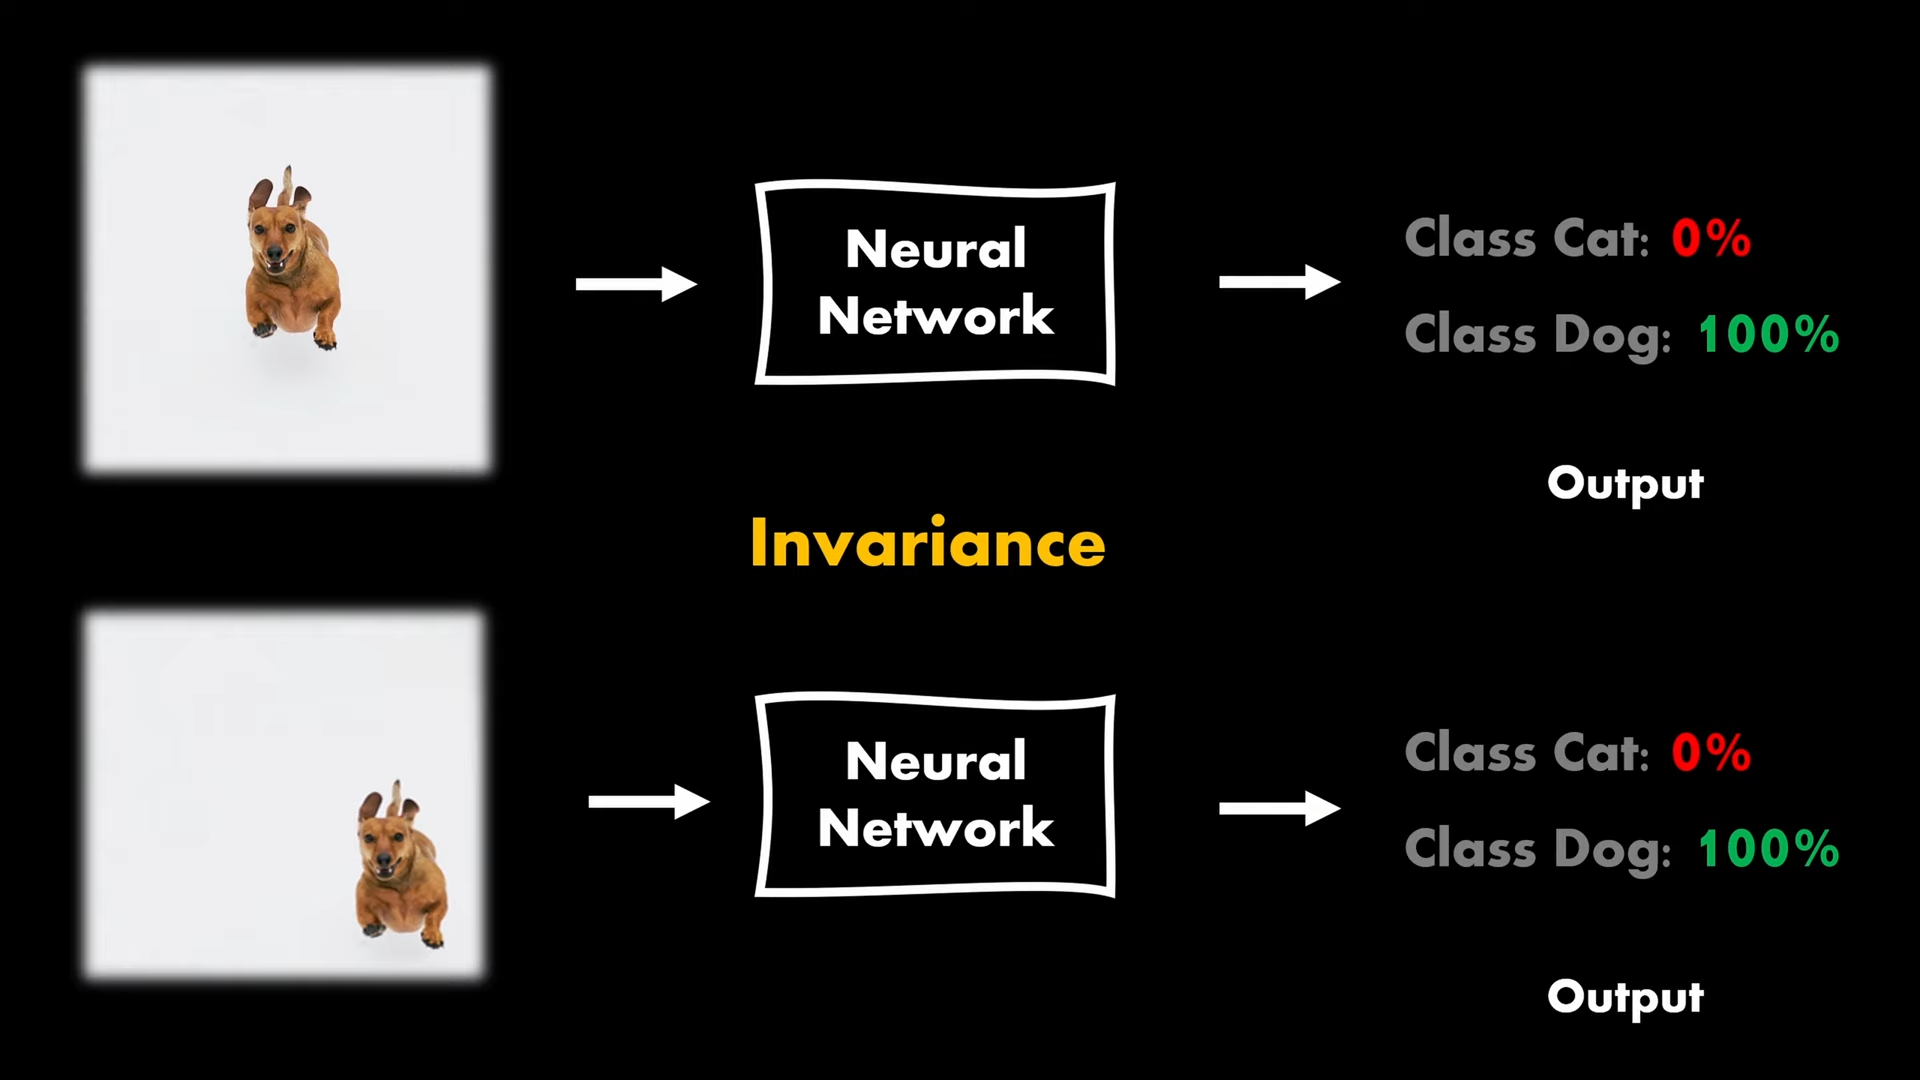
\includegraphics[scale=.2]{images/invariance}}
\end{figure}
\end{frame}

\begin{frame}
\frametitle{Equivariance}
\begin{figure}[h]
\centering{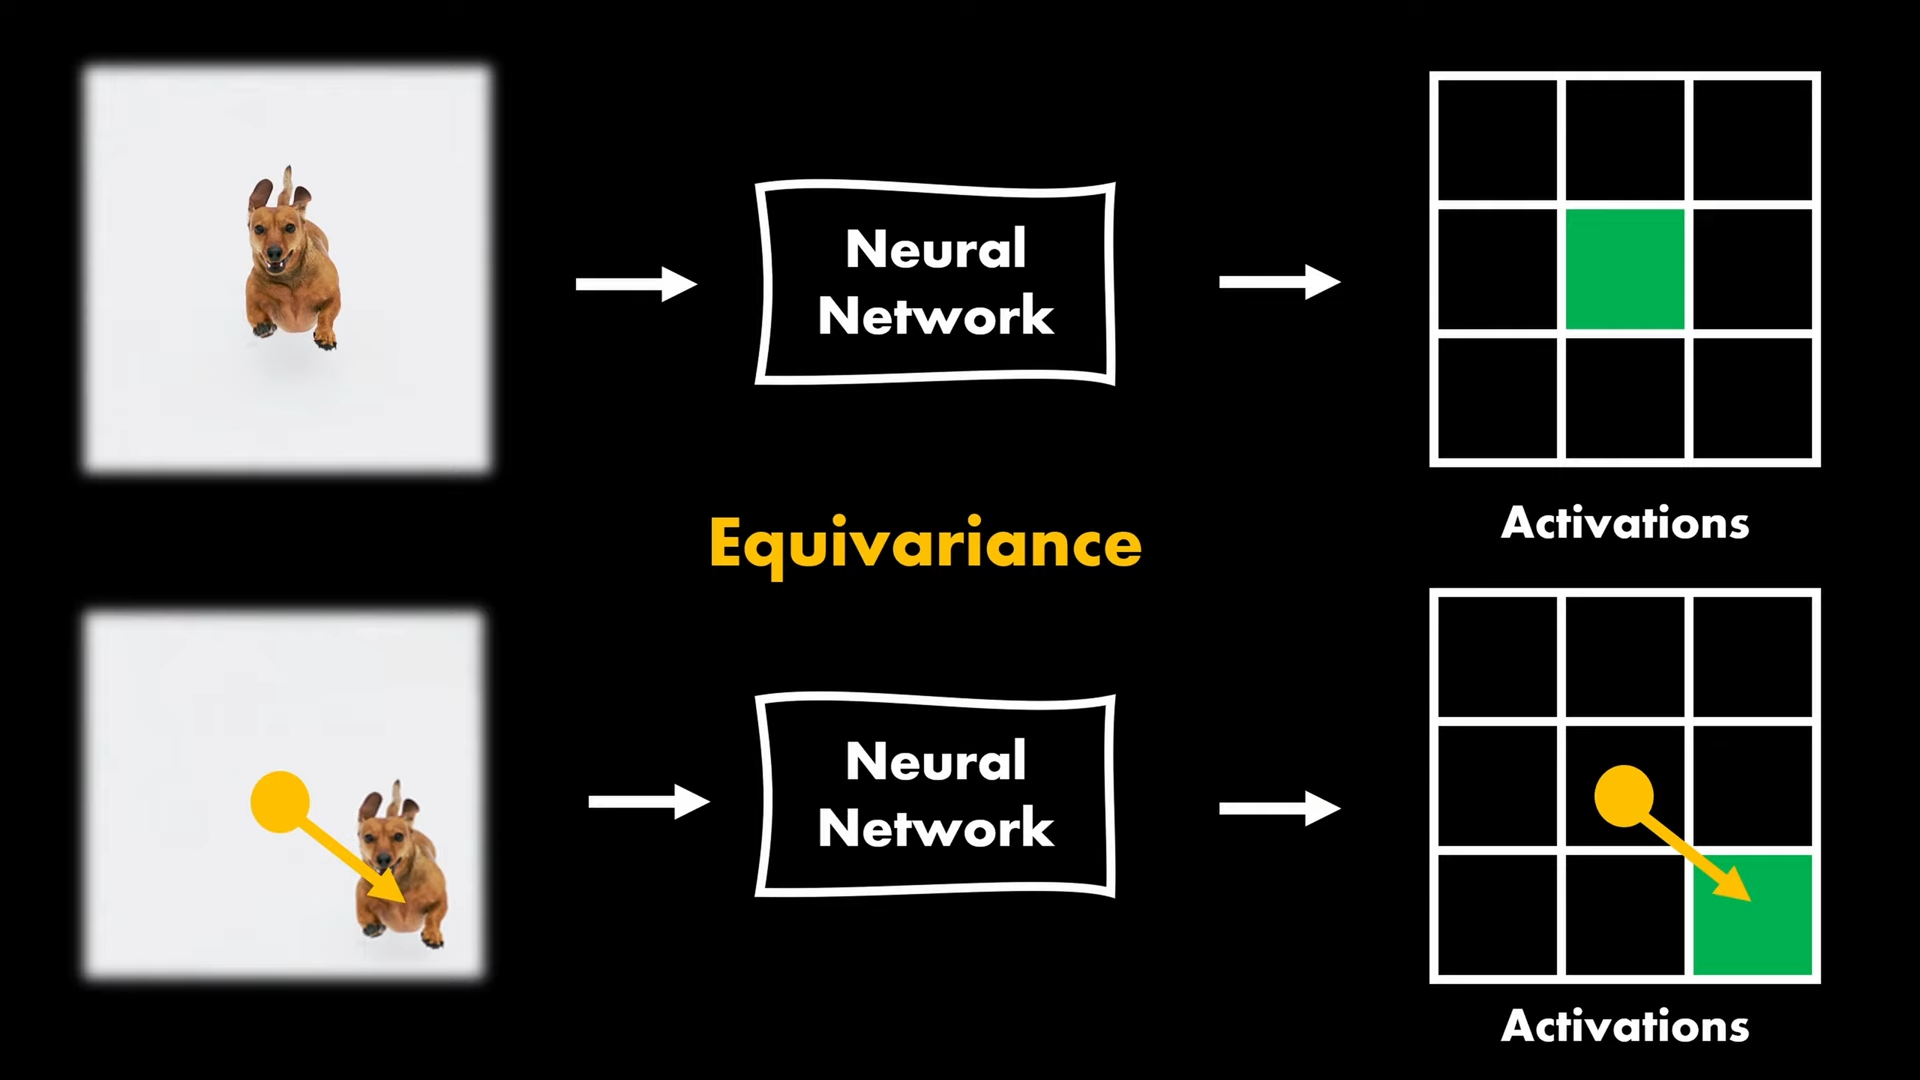
\includegraphics[scale=.2]{images/equivariance}}
\end{figure}
\end{frame}


\section{Frame Averaging}
\begin{frame}
\frametitle{Frame Averaging}
\begin{itemize}
\item<2-> Method to introduce equivariance and invariance to networks
\medskip
\item<3-> Averaging over subset of group instead of whole group
\medskip
\item<4-> Efficient and expressive
\end{itemize}
\end{frame}

\section{Outlook}
\begin{frame}
\frametitle{Outlook}
\begin{itemize}
\item<2-> Introduce layer-wise equivariance in decoder
\medskip
\item<3-> Each layer represents features
\medskip
\item<4-> Mesh $\rightarrow$ Mesh
\end{itemize}
\end{frame}

\end{document}